
\definecolor{purple2}{RGB}{218,112,214}

Now that enough is known about numbers, it is possible to work with non-numbers. The only known non-numbers at this point are the switches. But is knowing what they are enough to playing them? The game simpler cashing cheques will tell.

In this game there is a table with purple cheques. Each cheque has two numbers written on top, and, in each player's turn they will either pay one coin or cash a cheque that will grant him a number of coins equal to the correspondent associated integer. What is the best move for left?

\begin{center}
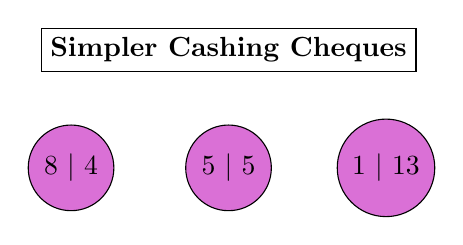
\begin{tikzpicture}
	\node[draw] (title) at (0,1.5) {\textbf{Simpler Cashing Cheques}};
	\begin{scope} [every node/.style={style=circle, draw, fill=purple2}]
		\node at (-2,0) {8 $|$ 4};
		\node at (0,0) {5 $|$ 5};
		\node at (2,0) {1 $|$ 13};
	\end{scope}
\end{tikzpicture}
\end{center}

Definitely the move is not paying as left can earn money in his turn. A good thing to grasp from this example is that you should never play in a number, paying a coin in this case, if there are non-numbers, cashing a purple cheque in this case. Should left cash 8, 5 or 1? 1, of course. The reader is encouraged to play as left and trying to find the best possible outcome, but the answer is playing the hottest switch. Although the game above is not a switch, it is a sum of switches, and, because of that can benefit of the simplified notation discussed earlier.

\begin{align*}
	G =& (\frac{8-4}{2} \pm \frac{8+4}{2}) + (\frac{5-5}{2} \pm \frac{5+5}{2}) + (\frac{1-13}{2} \pm \frac{1+13}{2}) \\
	  =& (2 \pm 6) + (0 \pm 5) + (-6 \pm 7)\\
	  =& -4 \pm 7 \pm 6 \pm 5
\end{align*}

If you analyze the result above, it becomes clear that left must play on the rightmost component as, although it will not provide many coins, it will prevent right from cashing a huge amount. It is very possible to build scenarios where a player would even pay for cashing a cheque if that prevented the opponent from getting rich. Now that playing a simpler cashing cheques became easy, a more challenging task will rise. How to play Domineering well?

Playing a game like Domineering well involves the concepts of \defi{left/right stops}, \defi{toenail}, \defi{ambient temperature}, \defi{freezing point} and, to put all that together, \defi{thermograph}.

\begin{center}
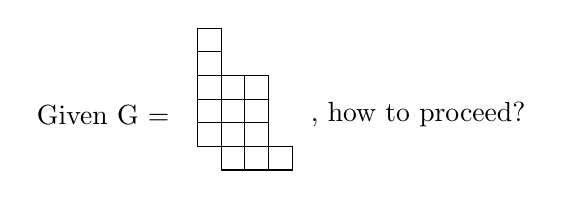
\begin{tikzpicture}
	\node at (-1.5,0.1) {Given G =};
	\draw[] (0,-0.6) rectangle ++(0.3,0.3);
	\draw[] (0.3,-0.6) rectangle ++(0.3,0.3);
	\draw[] (0.6,-0.6) rectangle ++(0.3,0.3);
	\draw[] (-0.3,-0.3) rectangle ++(0.3,0.3);
	\draw[] (0,-0.3) rectangle ++(0.3,0.3);
	\draw[] (0.3,-0.3) rectangle ++(0.3,0.3);
	\draw[] (-0.3,0) rectangle ++(0.3,0.3);
	\draw[] (0,0) rectangle ++(0.3,0.3);
	\draw[] (0.3,0) rectangle ++(0.3,0.3);
	\draw[] (-0.3,0.3) rectangle ++(0.3,0.3);
	\draw[] (0,0.3) rectangle ++(0.3,0.3);
	\draw[] (0.3,0.3) rectangle ++(0.3,0.3);
	\draw[] (-0.3,0.6) rectangle ++(0.3,0.3);
	\draw[] (-0.3,0.9) rectangle ++(0.3,0.3);
	\node at (2.5,0.1) {, how to proceed?};
\end{tikzpicture}
\end{center}

\begin{center}
	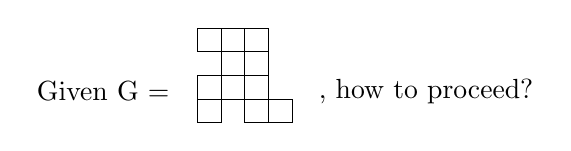
\begin{tikzpicture}
		\node at (-1.2,0.1) {Given G =};
		\draw[] (0.6,-0.3) rectangle ++(0.3,0.3);
		\draw[] (0.9,-0.3) rectangle ++(0.3,0.3);
		\draw[] (0,-0.3) rectangle ++(0.3,0.3);
		\draw[] (0,0) rectangle ++(0.3,0.3);
		\draw[] (0.3,0) rectangle ++(0.3,0.3);
		\draw[] (0.6,0) rectangle ++(0.3,0.3);
		\draw[] (0.3,0.3) rectangle ++(0.3,0.3);
		\draw[] (0.6,0.3) rectangle ++(0.3,0.3);
		\draw[] (0,0.6) rectangle ++(0.3,0.3);
		\draw[] (0.3,0.6) rectangle ++(0.3,0.3);
		\draw[] (0.6,0.6) rectangle ++(0.3,0.3);
		\node at (2.9,0.1) {, how to proceed?};
	\end{tikzpicture}
\end{center}

G is definitely not a switch nor a sum of switches. It is possible to say the temperature in G is going to stay high for quite some time, although there is no definition for that yet, simply because hotness is term used to define the importance of the next move. A good place to start is writing out the game tree.

\begin{figure} [!ht]
\begin{center}
\begin{tikzpicture}
	[
	sibling distance=150pt,
	level distance=100pt,
	level 1/.style={sibling distance=4cm},
	level 2/.style={sibling distance=1.7cm},
	every node/.style = {
	},
	every child/.style = {
		ultra thick
	}
	]

\node[draw] (title) at (0, 1) {Game Tree};

\node {
	\begin{tikzpicture}
		\draw[] (0.6,-0.6) rectangle ++(0.3,0.3);
		\draw[] (0.3,-0.6) rectangle ++(0.3,0.3);
		\draw[] (0.9,-0.6) rectangle ++(0.3,0.3);
		\draw[] (0,-0.6) rectangle ++(0.3,0.3);
		\draw[] (0,-0.3) rectangle ++(0.3,0.3);
		\draw[] (0.3,-0.3) rectangle ++(0.3,0.3);
		\draw[] (0.6,-0.3) rectangle ++(0.3,0.3);
		\draw[] (0.9,-0.3) rectangle ++(0.3,0.3);
	\end{tikzpicture}}
child[blue, level distance=80pt] {node[black] {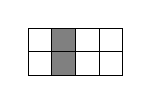
\begin{tikzpicture}
			\draw[] (0.6,-0.6) rectangle ++(0.3,0.3);
			\draw[fill=gray] (0.3,-0.6) rectangle ++(0.3,0.3);
			\draw[] (0.9,-0.6) rectangle ++(0.3,0.3);
			\draw[] (0,-0.6) rectangle ++(0.3,0.3);
			\draw[] (0,-0.3) rectangle ++(0.3,0.3);
			\draw[fill=gray] (0.3,-0.3) rectangle ++(0.3,0.3);
			\draw[] (0.6,-0.3) rectangle ++(0.3,0.3);
			\draw[] (0.9,-0.3) rectangle ++(0.3,0.3);
	\end{tikzpicture}}
	child[blue] {node[black] {\gam{1}{}}}
	child[blue] {node[black] {\gam{1}{{-}1}}}
	child[red, dashed] {node[black] {\gam{{-}1}{1}}}
}
child[blue] {node[black] {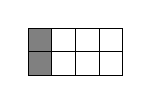
\begin{tikzpicture}
			\draw[] (0.6,-0.6) rectangle ++(0.3,0.3);
			\draw[] (0.3,-0.6) rectangle ++(0.3,0.3);
			\draw[] (0.9,-0.6) rectangle ++(0.3,0.3);
			\draw[fill=gray] (0,-0.6) rectangle ++(0.3,0.3);
			\draw[fill=gray] (0,-0.3) rectangle ++(0.3,0.3);
			\draw[] (0.3,-0.3) rectangle ++(0.3,0.3);
			\draw[] (0.6,-0.3) rectangle ++(0.3,0.3);
			\draw[] (0.9,-0.3) rectangle ++(0.3,0.3);
	\end{tikzpicture}}
	child[blue] {node[black] {\gam{1}{}}}
	child[blue] {node[black] {\gam{1}{{-}1}}}
	child[red, dashed] {node[black] {\gam{{-}1}{0,1}}}
}
child[red, dashed, level distance=80pt] {node[black, solid] { 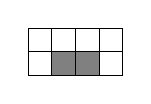
\begin{tikzpicture}
			\draw[fill=gray] (0.6,-0.6) rectangle ++(0.3,0.3);
			\draw[fill=gray] (0.3,-0.6) rectangle ++(0.3,0.3);
			\draw[] (0.9,-0.6) rectangle ++(0.3,0.3);
			\draw[] (0,-0.6) rectangle ++(0.3,0.3);
			\draw[] (0,-0.3) rectangle ++(0.3,0.3);
			\draw[] (0.3,-0.3) rectangle ++(0.3,0.3);
			\draw[] (0.6,-0.3) rectangle ++(0.3,0.3);
			\draw[] (0.9,-0.3) rectangle ++(0.3,0.3);
	\end{tikzpicture}}
	child[blue, solid] {node[black] {\gam{{-}1}{0, 1}}}
	child[red] {node[black] {\gam{1}{}}}
	child[red] {node[black] {\gam{0}{0}}}
}
child[red, dashed] {
	node[black, solid] { 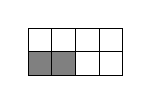
\begin{tikzpicture}
	\draw[] (0.6,-0.6) rectangle ++(0.3,0.3);
	\draw[fill=gray] (0.3,-0.6) rectangle ++(0.3,0.3);
	\draw[] (0.9,-0.6) rectangle ++(0.3,0.3);
	\draw[fill=gray] (0,-0.6) rectangle ++(0.3,0.3);
	\draw[] (0,-0.3) rectangle ++(0.3,0.3);
	\draw[] (0.3,-0.3) rectangle ++(0.3,0.3);
	\draw[] (0.6,-0.3) rectangle ++(0.3,0.3);
	\draw[] (0.9,-0.3) rectangle ++(0.3,0.3);
	\end{tikzpicture}}
		child[blue, solid] {node[black] {\gam{{-}1}{1}}}
		child[blue, solid] {node[black] {\gam{{-}1}{0,1}}}
		child[red] {node[black] {\gam{}{{-}1}}}
	}
;

\end{tikzpicture}
\end{center}
\end{figure}

blabla


